\newpage
\section{HM.API}
Zur Implementierung der REST \ac{api} wird die \textit{HttpListener} Klasse verwendet. Diese Klasse stellt einen HTTP-Protokollistener zur Verfügung, welcher auf die \ac{http}-Anfragen antwortet. \cite{HttpListener}\\
Die \textit{HttpListener} Klasse wird von der \textit{DataBaseAPI} Klasse, im \textit{HM.API} Verzeichnis, abstrahiert. Des Weiteren referenziert die \textit{DataBaseAPI} Klasse das in Abschnitt \ref{sec:HMDBServices} beschriebene \textit{HM.DBServices} Verzeichnis und verwendet hierbei die \textit{SQLiteWrapper} und \textit{ConfigurationReader} Klassen. Zudem wird die Variable \textit{Targets} definiert, welche eine Liste von zur Auswahl stehenden Datensätze repräsentiert. Die Instanzen der Klassen werden anschließend im Konstruktor der Klasse erzeugt.\\
Um die Plattformunabhängigkeit des Systems beizubehalten wird in der \textit{InitTargets()} Funktion der Klasse die \textit{Targets} Liste, abhängig von der in der Konfigurationsdatei gesetzten Plattform erstellt. Hierbei wird ein \textit{Target} Objekt an die \textit{Targets} Liste hinzugefügt. Dieses setzt sich aus den Parametern \textit{dwReadingID}, \textit{szLabelUser} und \textit{tableName} zusammen und wird dazu verwendet, die richtigen Datensatz in der Datenbank ausfindig zu machen.\\
Sollen weitere Datensätze des Hardware-Health-Monitors über die \ac{api} zugängig gemacht werden, müssen diese in der in Listing \ref{lst:InitTargets} aufgeführten \textit{InitTargets()} Funktion hinzugefügt werden. 
\begin{lstlisting}[caption={InitTargets Funktino der DataBaseAPI}, label={lst:InitTargets}]
    List<Target> Targets;
    private void InitTargets()
    {
        Targets = new List<Target>();
        switch (config.deviceType)
        {
            case "FLX":
                Targets.Add(new Target("16777217", "Temperature 1", "TempReadings"));
                ...
                break;
            case "OfficePC":
                Targets.Add(new Target("16777470", "CPU Package", "TempReadings"));
                ...
                break;
        }
        Targets.Add(new Target("latest", "CurrentSystemStatus", "SystemStatus"));
        Targets.Add(new Target("latest", "SystemStatusHistory", "HistorySystemStatus"));
        Targets.Add(new Target("latest", "SystemReliability", "SystemReliability"));

    }
\end{lstlisting}
\subsection{Bearbeitung der \ac{http}-Anfragen}
\begin{wrapfigure}{r}{0.55\textwidth}
    \vspace{-1.2cm}
    \begin{center}
      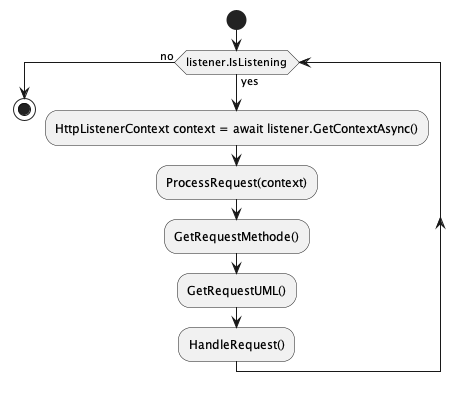
\includegraphics[width=0.55\textwidth]{APIAblauf.png}
    \end{center}
    \vspace{-0.5cm}
    \caption{Ablauf der Requestbehandlung}
    \label{fig:APIAblauf}
    \vspace{-0.5cm}
  \end{wrapfigure}
Wird eine Anfrage an die \ac{api} gestellt, durchläuft diese eine Reihe von Switch Anweisungen, welche sie nach Methode (GET, POST, etc.) und URL sortieren. Hierzu wird zunächst in der \textit{ProcessRequest()} Funktion die Anfrage (Request) dem Listenercontext entnommen. Anschließend wird der Typ der Anfrage ermittelt.\\
Durch die Schnittstellenbeschreibung in \cite{SimpleJSON} werden keine GET Anfragen vom Grafanadashboard versendet. Daher werden alle gestellten GET Anfragen von der \ac{api} mit der Nachricht \glqq\textit{No Implementation}\grqq{} beantwortet.\\
Jede POST Anfragen geht durch eine weitere Switch Anweisung. Hierbei wird nach der URL der Anfrage sortiert. Anschließend wird das angefragte Zeitintervall, so wie das Target, dem Body der Anfrage entnommen. Über die \textit{SQLiteWrapper} Klasse werden passende Datensätze ausgelesen und in die Antwort der \ac{api} eingebaut.\\   
Die Antworten der \ac{api} werden im \ac{json} Format zurückgesendet. Dabei werden grundsätzlich drei Typen von Antworten versendet. Die Antwort auf eine \textit{/search}-Anfrage, liefert eine Liste von zur Auswahl stehenden Datensätzen. Diese wird bei der Konfiguration der Datenquelle (Siehe Abbildung \ref{fig:PanelBearbeitung}) an die \ac{api} versendet. Anschließend werden die Datensätze der Datenbank über die \textit{/query}-Anfrage angefragt. Die Antwort ist dabei abhängig von dem angefragten Datenformat. Die Datensätze können hierbei entweder als \textit{Table} oder \textit{TimeSeries} versendet werden.\\
Im Folgenden werden die Konfigurationen der Antworten, im \ac{json} Format, aufgeführt:
\begin{enumerate}
    \item \textbf{/search}\\
    \begin{lstlisting}[caption={\glqq/search\grqq{} Response}, label={lst:search}]
    ["Temperature 1","CPU Load","CurrentSystemStatus","SystemStatusHistory","SystemReliability"]
    \end{lstlisting}
    \item \textbf{/query - Timeseries}\\
    \begin{lstlisting}[caption={/query-Timeseries Response}, label={lst:queryTimeseries}]
        [{
            "target":"Temperature 1", 
            "datapoints":[
              [64,1450754160000],  
              [65,1450754220000],
              ...
            ]
        }]
    \end{lstlisting}
    \item \textbf{/query - Table}\\
    \begin{lstlisting}[caption={/query-Table Response}, label={lst:queryTable}]
        [{
            "columns":[
                {"text":"Optimal","type":"number"},
                {"text":"Elevated","type":"number"},
                {"text":"Critical","type":"number"}
            ],
            "rows":[
                [0.5,0.25,0.25],
            ],
            "type":"table"
        }]
    \end{lstlisting}
\end{enumerate}





%\textbf{/search} Anfragen\\
%Die Antwort auf eine \textit{/search} Anfrage, setzt sich aus den \textit{szLabelUser} Parametern der \textit%{Targets}-Liste zusammen und ist dabei wie Folgt aufgebaut:
%\begin{lstlisting}[caption={\glqq/search\grqq{} Response}, label={lst:search}]
%["Temperature 1","CPU Load","CurrentSystemStatus","SystemStatusHistory","SystemReliability"]
%\end{lstlisting}
%\vspace{-0.9cm}
%
%
%
%Die Antwort auf eine \textit{/query} Anfrage ist abhängig von Typ des Targets. Hierbei wird zwischen \textit%{TimeSeries} und \textit{Table} unterschieden.\\
%Die Antworten der \textit{/query} werden sehen wie folgt aus:
%\vspace{-1cm}
%\subsubsection*{TimeSeries}
%\begin{lstlisting}[caption={/search-Timeseries Response}, label={lst:queryTimeseries}]
%[{
%    "target":"Temperature 1", 
%    "datapoints":[
%      [64,1450754160000],  
%      [65,1450754220000],
%      ...
%    ]
%}]
%\end{lstlisting}
%\vspace{-1.5cm}
%\subsubsection*{Table}\todo{Anpassen für SystemStatus oder sowas}
%\begin{lstlisting}[caption={/search-Table Response}, label={lst:queryTable}]
%[
%    {
%      "columns":[
%        {"text":"Time","type":"time"},
%        {"text":"Country","type":"string"},
%        {"text":"Number","type":"number"}
%      ],
%      "rows":[
%        [1234567,"SE",123],
%        [1234567,"DE",231],
%        ...
%      ],
%      "type":"table"
%    }
%]
%\end{lstlisting}
%\vspace{-0.9cm}